\chapter{Results}

This chapter presents the results of the analysis performed using the framework. Keep in mind that POX isn't designed to compete with the very best (cite POX's own graphs showing it's worse than NOX), but is designed for academia. Given that, none of this will be compared with existing industry-standard controllers such as Beacon or OpenDaylight (what is with all the light metaphors?).

Also all testing will be done entirely in software, no real switches will be used.

\section{Comparison of Routing Metrics}
Analysis goes here. dunno what to call this, routing performance or whatever. something title-capsy.


\begin{table}
\caption{Summary of incredible achievements}
\end{table}

\begin{figure}
\centering
\documentclass[preview=false]{standalone}

\usepackage{color}
\usepackage{tikz}
\usepackage{pgfplots}
\definecolor{mcfblue}{rgb}{0,0.8,1}
\definecolor{mcforange}{rgb}{1,0.6,0}
\definecolor{mcfgreen}{rgb}{.68,.81,0}
\definecolor{mcfgrey}{gray}{0.95}
\definecolor{mcforange2}{rgb}{1,0.8,0}
\definecolor{mcforange3}{rgb}{1,0.2,0}

\begin{document}

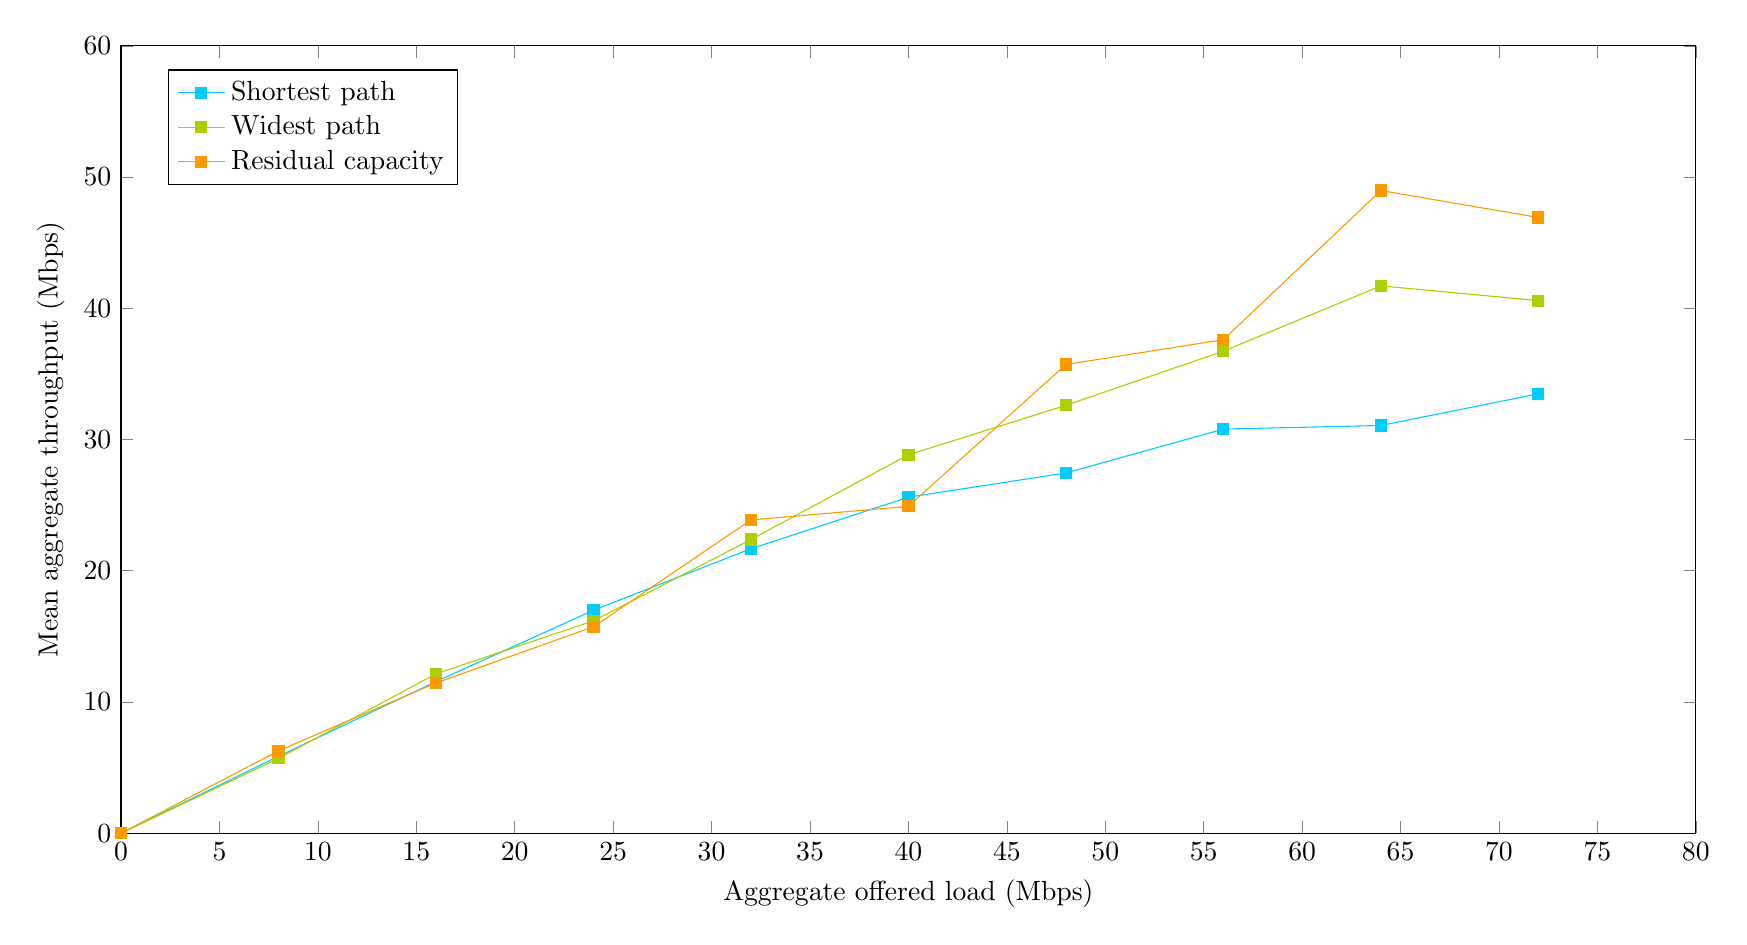
\begin{tikzpicture}
  \begin{axis}[
    width = 20cm,
    height = 10cm,
    xlabel = Aggregate offered load (Mbps),
    ylabel = Mean aggregate throughput (Mbps),
    xmin=0, xmax=80, ymin=0, ymax=60,
    scale only axis,
    legend pos=north west,
    legend cell align=left
  ]

  \addplot[
    mark=square*, mcfblue, draw=mcfblue, 
    %error bars/.cd, y dir=both, y explicit
  ]
  table[x=x,y=y,y error=yerr]
  {
    x       y        yerr
    0 0 0
    8 5.86176695  0.8231965435
    16  11.5535775  1.8500848174
    24  16.9892942  2.7284167978
    32  21.6772777  3.1246555125
    40  25.60601145 4.6067375898
    48  27.4505014  4.268460193
    56  30.79341035 5.1600664391
    64  31.0690037  3.1123100166
    72  33.482466 4.9881937497
  };
  \addlegendentry{Shortest path}

  \addplot[
    mark=square*, mcfgreen, draw=mcfgreen,
    %error bars/.cd, y dir=both, y explicit
  ]
  table[x=x,y=y,y error=yerr]
  {
    x       y        yerr
    0 0 0
    8 5.70097005  0.9819427248
    16  12.1464775  1.959618983
    24  16.1806358  2.8838031317
    32  22.376414 3.157487707
    40  28.836408 4.2771214034
    48  32.6031681  5.1686668287
    56  36.731512 6.2149608988
    64  41.707273 5.0300720744
    72  40.5844955  6.9197951473
  };
  \addlegendentry{Widest path}


  \addplot[
    mark=square*, mcforange, draw=mcforange,
    %error bars/.cd, y dir=both, y explicit
  ]
  table[x=x,y=y,y error=yerr]
  {
    x       y        yerr
    0 0 0
    8 6.2758302105  0.9166252282
    16  11.449755 2.0397464764
    24  15.7299333  2.4486435236
    32  23.8737585  3.6694296596
    40  24.906494 4.0958964659
    48  35.71567985 6.2339491202
    56  37.6072411  5.6730688749
    64  48.971195 5.559440696
    72  46.91598  6.5831520159
  };
  \addlegendentry{Residual capacity}

  \end{axis}
\end{tikzpicture}

\end{document}

\caption{Aggregate throughput comparison for flow pattern `pairs'}
\label{fig:pairs}
\end{figure}

\begin{figure}
\centering
\documentclass[preview=false]{standalone}

\usepackage{color}
\usepackage{tikz}
\usepackage{pgfplots}
\definecolor{mcfblue}{rgb}{0,0.8,1}
\definecolor{mcforange}{rgb}{1,0.6,0}
\definecolor{mcfgreen}{rgb}{.68,.81,0}
\definecolor{mcfgrey}{gray}{0.95}
\definecolor{mcforange2}{rgb}{1,0.8,0}
\definecolor{mcforange3}{rgb}{1,0.2,0}

\begin{document}

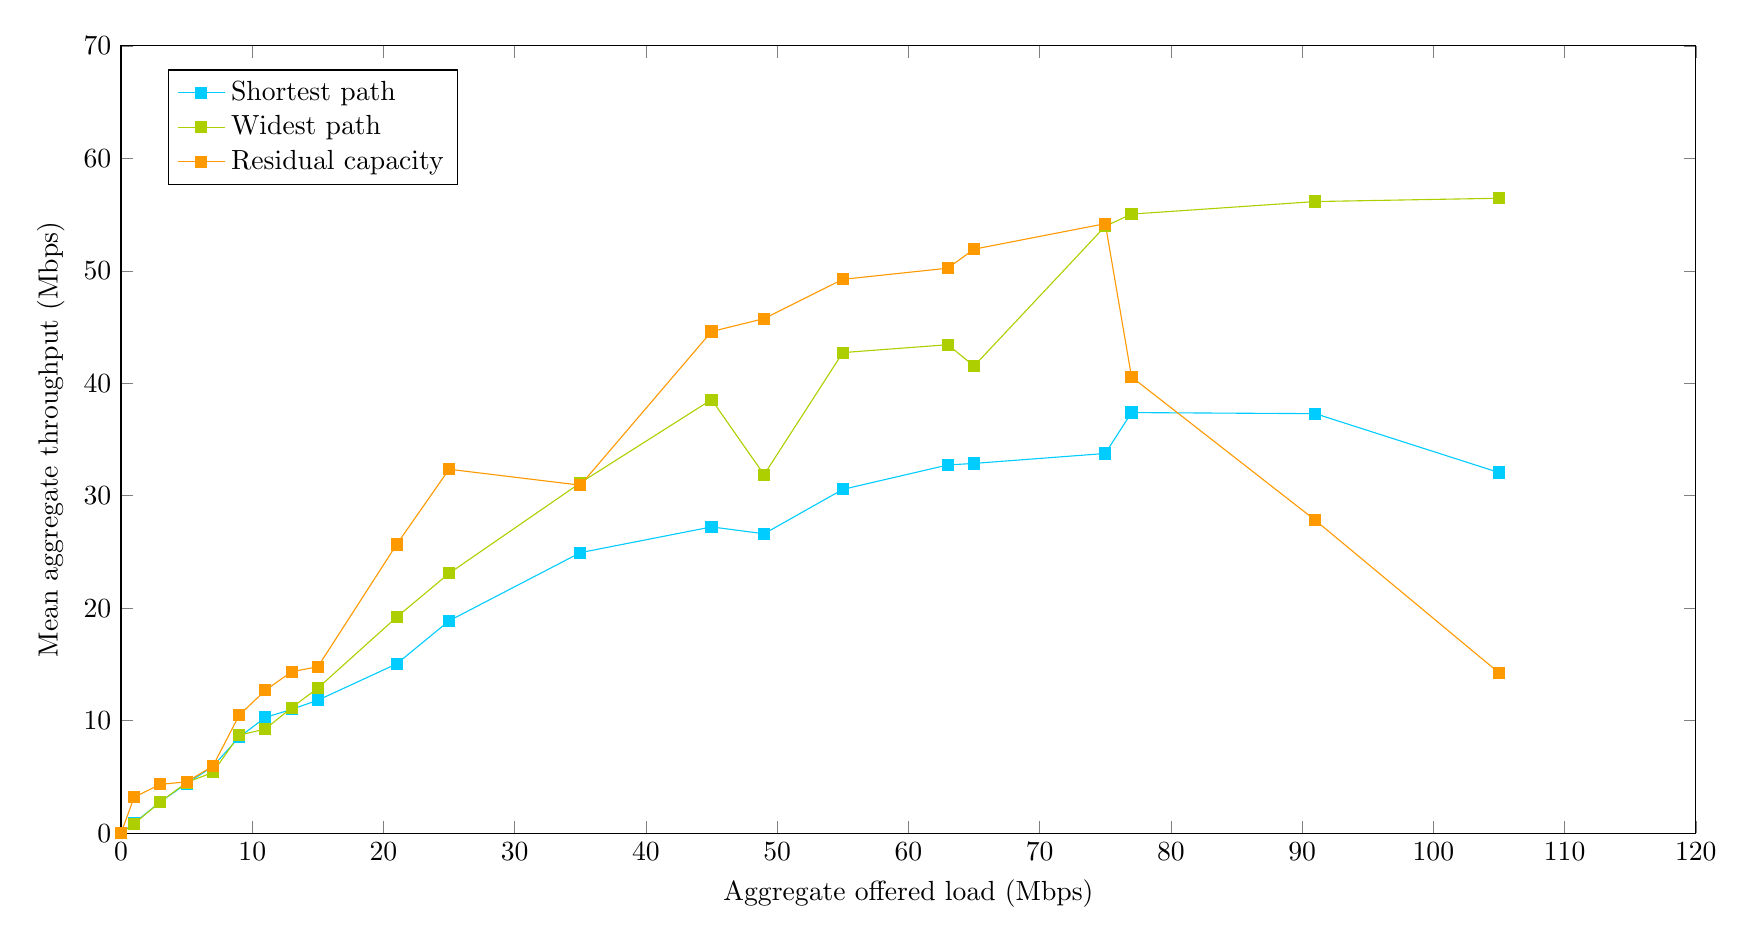
\begin{tikzpicture}
  \begin{axis}[
    width = 20cm,
    height = 10cm,
    xlabel = Aggregate offered load (Mbps),
    ylabel = Mean aggregate throughput (Mbps),
    xmin=0, xmax=120, ymin=0, ymax=70,
    scale only axis,
    legend pos=north west,
    legend cell align=left
  ]

  \addplot[
    mark=square*, mcfblue, draw=mcfblue, 
    %error bars/.cd, y dir=both, y explicit
  ]
  table[x=x,y=y]
  {
    x       y
    0 0
    0 0
    1 0.9076857333
    3 2.7887012
    5 4.4143781667
    7 5.9348530667
    9 8.5344292667
    11  10.2956094667
    13  11.0084661333
    15  11.8237655667
    21  15.0515486667
    25  18.8840666
    35  24.9408325333
    45  27.2294380667
    49  26.6205349333
    55  30.5667652667
    63  32.7360330667
    65  32.8748182667
    75  33.7584818667
    77  37.3938184
    91  37.2973111333
    105 32.0640434
  };
  \addlegendentry{Shortest path}

  \addplot[
    mark=square*, mcfgreen, draw=mcfgreen,
    %error bars/.cd, y dir=both, y explicit
  ]
  table[x=x,y=y]
  {
    x       y
    0 0
    0 0
    1 0.837472
    3 2.7918824
    5 4.5035344333
    7 5.4081212667
    9 8.7153884
    11  9.2621923333
    13  11.1652936667
    15  12.9007854333
    21  19.206016
    25  23.1014973333
    35  31.145868
    45  38.546948
    49  31.8722968
    55  42.7261178
    63  43.4277681333
    65  41.5316588667
    75  53.9628482667
    77  55.0400688667
    91  56.1537334
    105 56.4487925333
  };
  \addlegendentry{Widest path}


  \addplot[
    mark=square*, mcforange, draw=mcforange,
    %error bars/.cd, y dir=both, y explicit
  ]
  table[x=x,y=y]
  {
    x       y
    0 0
    0 0
    1 3.2083705
    3 4.3446018333
    5 4.56657
    7 5.9660251333
    9 10.48575505
    11  12.70449665
    13  14.3583371667
    15  14.7968646667
    21  25.66589895
    25  32.35605065
    35  30.9391424333
    45  44.5982052667
    49  45.7477358
    55  49.2379251333
    63  50.2314286333
    65  51.9199845
    75  54.18844885
    77  40.5596216833
    91  27.82448735
    105 14.2570914833
  };
  \addlegendentry{Residual capacity}

  \end{axis}
\end{tikzpicture}

\end{document}

\caption{Aggregate throughput comparison for flow pattern `random'}
\label{fig:random}
\end{figure}

\section{Scalability of Objective Functions}
The results sure were great.
well. they were pretty much as expected. discuss them i guess.
stats-gathering is really hard and it is sensitive to it. i think some people thought
about it but it's worth a whole thesis on its own really.
somewhat limited by not being able to discover link capacities (whatshisname is
doing his thesis on it so it’s a separate/big problem). meant had to use topos with
constant capacities and in practical terms identical capacities. considered writing a
thing to let you fake the topo too but w/ever.

\begin{figure}
\centering
\documentclass[preview=false]{standalone}

\usepackage{color}
\usepackage{tikz}
\usepackage{pgfplots}
\definecolor{mcfblue}{rgb}{0,0.8,1}
\definecolor{mcforange}{rgb}{1,0.6,0}
\definecolor{mcfgreen}{rgb}{.68,.81,0}
\definecolor{mcfgrey}{gray}{0.95}

\begin{document}

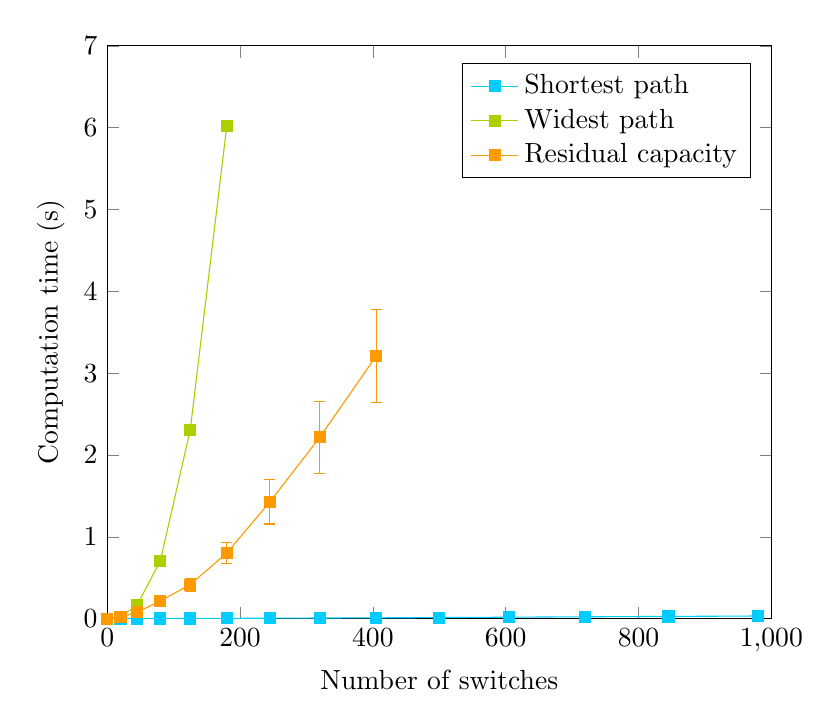
\begin{tikzpicture}
  \begin{axis}[
    xlabel = Number of switches,
    ylabel = Computation time (s),
    xmin=0, xmax=1000, ymin=0, ymax=7,
    scale only axis,
    legend pos=north east,
    legend cell align=left
  ]

  \addplot[
    mark=square*, mcfblue, draw=mcfblue, 
    error bars/.cd, y dir=both, y explicit
  ]
  table[x=x,y=y,x error=xerr,y error=yerr]
  {
    x       xerr    y        yerr
    0 0 0 0
    20  0 0.0004876 1.73519417885663E-005
    45  0 0.0008358 4.18849218990829E-005
    80  0 0.0014721333  6.19053392431026E-005
    125 0 0.0022006 7.2781235901969E-005
    180 0 0.0034614667  0.0001785953
    245 0 0.0051226 0.000218655
    320 0 0.0076167333  0.0002536135
    405 0 0.0097622 0.0004514924
    500 0 0.0126307333  0.0003758768
    605 0 0.0175304667  0.0007970859
    720 0 0.022809  0.0010120146
    845 0 0.0269979333  0.0012781702
    980 0 0.0321096667  0.0015394796
  };
  \addlegendentry{Shortest path}


  \addplot[
    mark=square*, mcfgreen, draw=mcfgreen,
    error bars/.cd, y dir=both, y explicit
  ]
  table[x=x,y=y,x error=xerr,y error=yerr]
  {
    x       xerr    y        yerr
    0 0 0 0
    20  0 0.0227468667  9.30541902746289E-005
    45  0 0.164329  0.0020093485
    80  0 0.706706  0.0081184043
    125 0 2.3045877333  0.0326936456
    180 0 6.0166279333  0.0497968407
  };
  \addlegendentry{Widest path}


  \addplot[
    mark=square*, mcforange, draw=mcforange,
    error bars/.cd, y dir=both, y explicit
  ]
  table[x=x,y=y,x error=xerr,y error=yerr]
  {
    x       xerr    y        yerr
    0 0 0 0
    20  0 0.0194374667  0.0023112736
    45  0 0.0774724667  0.0102995943
    80  0 0.2163074 0.0239292767
    125 0 0.4154031333  0.0805419029
    180 0 0.8022469333  0.1317485442
    245 0 1.4275060667  0.2714548502
    320 0 2.2149086667  0.4411705329
    405 0 3.2092397333  0.5724065512
  };
  \addlegendentry{Residual capacity}

  \end{axis}
\end{tikzpicture}

\end{document}

\caption{Comparison of routing algorithm scalability}
\label{fig:sca1}
Computation time is the time taken to route 16 random flows in Al-Fares fat-tree networks with increasing parameter $k$. Error bars show 95\% confidence intervals but are too small to be visible for the shortest path and widest path metrics. 
\end{figure}

\cite{fake}

These graphs only show the results of experiments on a certain class of topologies: ones with constant and therefore symmetrical link capacities. This was discussed earlier in section SECTION.


Running experiments on Mininet means that there are practical limitations of the system which limit the size of networks which can be emulated with Mininet; this limit is hit long before the scalability of objective functions becomes a factor. However, it is possible to test the scalability of individual objective functions without the surrounding framework, by passing mock network graphs and flow statistics to the function. 

The Al-Fares fat-tree is parametrisable by a parameter k, which indicates the number of ports per commodity switch used in the network; this produces a network with f(k) = SOMETHING switches and g(k) = SOMETHINGELSE hosts in total, and is therefore easy to scale up to large networks for scalability testing. In this test, flows were randomly generated between 16 random hosts, for Al-Fares networks starting from k = 4 until further tests became impractically slow to run (greater than X seconds).  The results of this testing are shown in figure FIGURE, for each of the three routing metrics under consideration.

As expected, the shortest-path metric scales extremely well. The basic algorithm is well-understood, and the particular implementation used here is the one provided with NetworkX, which includes a number of small optimisations as well.

The residual spare capacity implementation is based on the formulation described originally by Walkowiak. In his PAPER he gives the WHATEVER of the algorithm as O(crazy). As seen in section SECTION, the performance of the algorithm as a whole depends mostly on the number of possible paths in the network: for every, this must be considered. In its original form, the solution becomes unworkably slow (greater than X seconds) at k = 6 or SOMETHING, with just X switches considered; this corresponds to Y possible paths for any given source/destination pair. One major optimisation was therefore implemented: the length of possible paths considered is limited to 6 hops. This is enough hops to allow multiple paths to each aggregation and core switch, but not to bounce indefinitely and unnecessarily between the core and aggregation and aggregation and edge layers. Figure FIGURE demonstrates how much the scalability of the RSC metric is dependent on the maximum path length considered.

\begin{figure}
\centering
\documentclass[preview=false]{standalone}

\usepackage{color}
\usepackage{tikz}
\usepackage{pgfplots}
\definecolor{mcfblue}{rgb}{0,0.8,1}
\definecolor{mcforange}{rgb}{1,0.6,0}
\definecolor{mcfgreen}{rgb}{.68,.81,0}
\definecolor{mcfgrey}{gray}{0.95}
\definecolor{mcforange2}{rgb}{1,0.8,0}
\definecolor{mcforange3}{rgb}{1,0.2,0}

\begin{document}

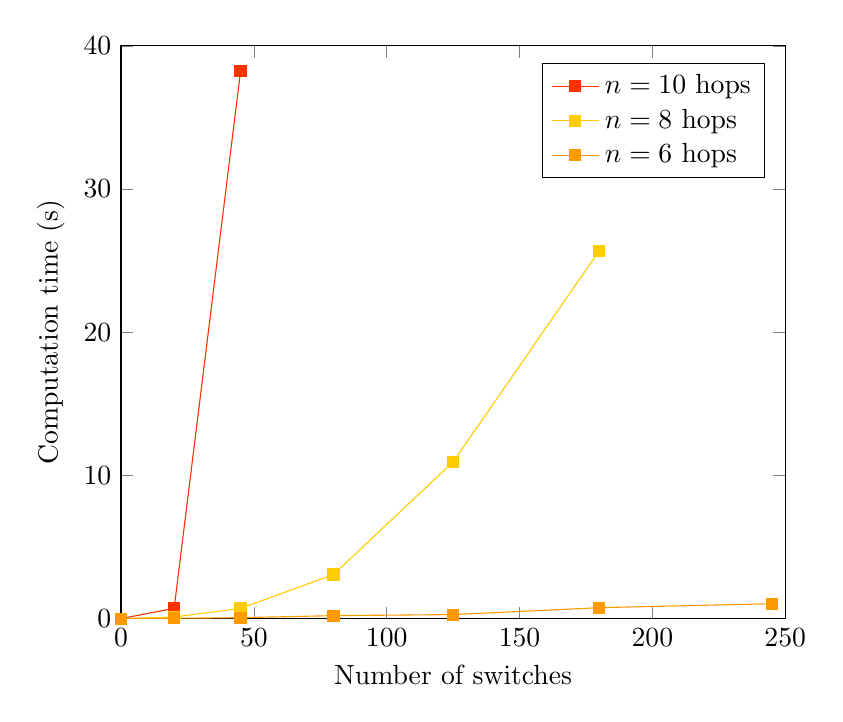
\begin{tikzpicture}
  \begin{axis}[
    xlabel = Number of switches,
    ylabel = Computation time (s),
    xmin=0, xmax=250, ymin=0, ymax=40,
    scale only axis,
    legend pos=north east,
    legend cell align=left
  ]

  \addplot[
    mark=square*, mcforange3, draw=mcforange3, 
    error bars/.cd, y dir=both, y explicit
  ]
  table[x=x,y=y,y error=yerr]
  {
    x       y        yerr
    0 0 0
    20  0.7256292 0.0070739045
    45  38.23024  0.1366292663
  };
  \addlegendentry{$n=10$ hops}

  \addplot[
    mark=square*, mcforange2, draw=mcforange2,
    error bars/.cd, y dir=both, y explicit
  ]
  table[x=x,y=y,y error=yerr]
  {
    x       y        yerr
    0 0 0 
    20  0.1143344 0.0027257511
    45  0.7122406 0.0030605062
    80  3.0836048 0.0217548799
    125 10.9429072  0.011007954
    180 25.692701 0.2385566181
  };
  \addlegendentry{$n=8$ hops}


  \addplot[
    mark=square*, mcforange, draw=mcforange,
    error bars/.cd, y dir=both, y explicit
  ]
  table[x=x,y=y,y error=yerr]
  {
    x       y        yerr
    0 0 0 
    20  0.0277476 0.0003812801
    45  0.06633 0.0036184659
    80  0.2110152 0.005928307
    125 0.283254  0.0053192575
    180 0.7664158 0.0074985986
    245 1.042033  0.0053563215
  };
  \addlegendentry{$n=6$ hops}

  \end{axis}
\end{tikzpicture}

\end{document}

\caption{Effect of maximum path length for residual capacity metric}
\label{fig:sca2}
Computation time is as for Figure \ref{fig:sca1}. Instead of considering all possible paths between hosts, only consider paths with a maximum path length of $n$ hops.
\end{figure}

The widest path metric performs quite poorly for such a well-known routing metric. The algorithm is based on a modified Dijkstra's algorithm, as described in section SECTION, which is not known to be particularly inefficient; the poor performance of the metric in these experiments is likely to be due to poor implementation. In particular, the algorithm must consider every path in the network, so, as for the RSC metric, the number of paths in an Al-Fares fat-tree can be very high and this is likely to be a significant factor in the algorithm's scalability. Unlike for RSC, however, limiting the number of paths considered was non-trivial due to the particular implementation, so this optimisation was not implemented. The dramatic effect of path length on the RSC metric seems to indicate that this would provide better scalability in this similar metric as well.

In this thesis, the objective function was only run once, the resulting throughput measured and the experiment stopped. Normally, the objective function would be run many times. It is quite impractical to try to globally optimise the entire network for every single new flow, and without letting the flow run for some time it is impossible to determine the demand, which is required to run the global optimisation anyway. In general, then, it seems that the approach used in this thesis would be reasonable: route flows initially along the shortest path, then every few seconds (as deemed appropriate; the gap would be shorter in a network mostly consisting of short bursts of traffic compared to large elephant flows) globally-optimal routes are recalculated.

In a normal scenario, however, the routing recalculation is performed every few seconds, and it is likely that many flows would be similar between calculations. This assumption can be made stronger if flows are consolidated; for example, group 'all HTTP traffic' along similar paths instead of calculating flow rules for individual 5-tuples, so that it is more likely that flows will average out to similar demands between calculations. In such an environment, recalculating the flow rules for the entire network from scratch becomes unreasonable. In many optimisation techniques, such as WHATEVER GLPK USES and simulated annealing as used in HEDERA, starting from an estimated solution which is close to the optimum greatly decreases the time taken to reach optimal levels; the previous calculation could be used as such an estimated solution. The implementation of this is non-trivial, and limits the use of third-party interfaces such as PuLP, since there is no way to specify a starting estimate for most solvers. Storing the state of, for example, the matrices used for linear algebra solutions to optimisation problems would be far more interesting. However, this is far outside the scope of this project and definitely in the realm of 'future work'.

From the perspective of this thesis, where the largest network considered was an Al-Fares fat-tree with k=4, the time taken to calculate routes is negligible for all routing metrics.


\section{Evaluation of Framework}

stuff about how great \thesis is
